\subsection{Challenges}
  \subsubsection{Filtered emails}
    One big design challenge we faced was how to reduce the number of irrelevant emails a student was receiving. Two solutions that were not optimal were discussed:
    \begin{itemize}
      \item \textbf{Opt in emails:} students could opt in for receiving certain email catagories based on tags. We soon realised that this would require a lot of maintence by students to continiously update their whitelist with tags as they were being created.
      Not only would it be a lot of work for a student, but students might miss out on exciting emails which do not fall into specific catagories, or a catagory a student had remembered to whitelist. For example the Raspberry Pie is unlikely to fall into a tag group but it's own. If a student forgets to add this to their list they'll miss out entirely on the emails when the likilihood is that they may have been interested.
      \item \textbf{Opt out emails:} students can blacklist tags that they never want to hear from. If an email contains a tag that a student has blacklisted then the student will never get sent this email. Whilst this is a lot closer to our ideal solution we still have the case of a student being interested in C++ say, but blacklisting Java. If an email contains two sections about these two languages and is labelled as containing both the student will never receive the email since Java was in their blacklist.
    \end{itemize}

    We have therefore devised a hybrid solution:
    \begin{itemize}
      \item A student will \textbf{receive} an email if none of the email tags fall in a students blacklist.
      \item A student will \textbf{receive} an email if one or more email tags fall in their blacklist but a tag in the emails list exists in their skill set.
      \item A student will \textbf{not receive} emails from a company they have blocked unless they have signed up to an event in which case they will \textbf{receive} the event related emails only.
      \item A student will \textbf{not receive} an email if any of the tags exist in the emails tags and none exist in the students skill set.
    \end{itemize}

    Furthermore in the student account settings we allow them to choose between receiving this smart email system, all emails, or only personal and event emails.

  \subsubsection{Intuative Features}
    Since it is not feasible to write a user manual for a website we faced many challenges ensuring that each user finds our site easy to navigate through and is made aware very quickly about the features that are available to them. Since we developed the site it is obvious to us how to use it but to ensure that users know too we have made use of the following:

    \paragraph{Tooltips:} These appear whenever you run your cursor over an area of text that can be edited in place, or over features that might not be completely obvious (such as company conact card drag and drop). Examples are the students name, year, degree, and bio. They all start with `click here to' and we believe they are well placed and helpful rather than irritating.      
    \begin{figure}[H]\centering
    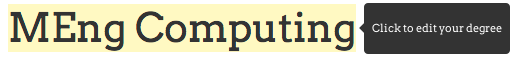
\includegraphics[scale=0.5]{images/design/edit_degree_tooltip}
    \caption{Useful degree tooltip}
    \end{figure}
    Tooltips also appear throughout for both company and department administrators.
    Once a user is comfortable with using the site, they have the option to turn tooltips off in their settings.

    \paragraph{Yellow Highlighting:} This also ties in nicely with the tooltips and highlights the boundary for what can and cannot be edited.

    \paragraph{Incomplete Sections:} In order to highlight to any user a section, document or field that is incomplete we have opted to highlight these in red rather than providing a message. We feel that by keeping this theme consistent throughout all users profiles it is quite intuative in itself.
    Whats more is that when a student initially signs up they are informed that their profile is inactive and they need to fill in certain fields before they can activate it. As they fill in these fields (which are initially red) the colour dissapears and we hope that students will intuatively learn from the beginning that the red colouring means an item is missing.

    \paragraph{Typeahead} Unfortunately there are too many degree types throughout departments for us to validate. For example just within the Department of Computing we have BEng, MEng, PhD, MSc and within these we have specialist titles such as Artificial Intelligence, Software Engineeing, Computation in Biology and Medicine etc.\cite{doc-ug-degrees}. In order to achieve our objective of being available to multiple departments it is just not possible to validate these. Therefore in order to try to ensure students doing the same degree have the same title (i.e. `MEng Computing' rather than `MEng computing' or `meng computing' etc.) we have used Twitter Bootstraps typeahead feature which provides options for students to choose from on typing. They will hopefully feel encouragd to click on these options. The options are populated from the list of degrees that students throughout the department are currently using on their profiles and so is very dynamic.

    \begin{figure}[H]\centering
    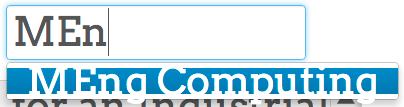
\includegraphics[scale=0.5]{images/design/edit_suggestions}
    \caption{Drop down degree suggestor}
    \end{figure}

    Likewise we make use of typeaheads throughout our site when allowing tag input. The aim of this is to make users aware of the tags available to them on input. This is again dynamically populated from the list of students tags, and if a tag is not in the list students have the option to add a new one by simply typing it in the tag input field. 

    We decided that only students should be allowed to add new tags, companies can only tag their emails with tags that exist in the system to aid with the smart email filtering.
    All tags are automatically downcased both on the server and the client.

    \paragraph{Navigation:} This has largely been made possible through the use of a navigation bar at the top of our website. We feel that this is intuative to all of our users who will be familiar with navigation bars from other sites such as Facebook\cite{facebook}, LinkedIn\cite{linkedin} and even Google\cite{google}. These websites really encourage user interaction by clicking on items located anywhere on the page and adopt the technique of changing the cursor to a pointer (hand) rather than the default which is normally displayed when you can interact with an object. As such we've adopted this technique through our site when items on the page can be clicked on to redirect. For example students can click on the top three events \& placements that are displayed on their dashboard. In order to make it very obvious we subtly change the colour scheme of the background to display that they've highlighted it.
    % TODO INSERT PICTURE HERE

    We have also made use of icons in order to make navigation more intuative, again users of every day websites have become accustimed to certain items meaning certain things, for example a cog is often associated with settings and so we had no qualms about using them freely in the design of our site.
    The downwards facing caret is used to alert users that clicking on their name on the navigation bar provides them with extra options.
    
    \begin{figure}[H]\centering
    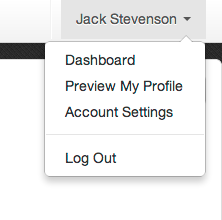
\includegraphics[scale=0.5]{images/design/navigation_caret}
    \caption{Drop down menu, intention aided by dropdown caret}
    \end{figure}

    Similarly the star and ban icons on a company as featured earlier, combined with the tooltips make it clear to a user what they mean.